\documentclass[12pt]{article}
\usepackage[english]{babel}
\usepackage[utf8]{inputenc}
\usepackage{amsmath, amssymb,amsthm}
\usepackage{graphicx}
\usepackage{hyperref}
\usepackage{geometry}

\graphicspath{{./images/}}
\setlength{\topmargin}{0pt}
\setlength{\headsep}{0pt}
\textheight = 600pt

\title{Probability Theory \\ Daily Task}
\author{Ben Kallus}
\date{October 5, 2020}

\begin{document}
\maketitle

$$f_Y(y) = \begin{cases} cy & \text{if}~0 \leq y \leq 1, \\
                         0 & \text{else.} \end{cases}$$

\noindent{\bf 1.}
\begin{align*}
    \int_{-\infty}^\infty f_Y(y)\,dy &= 1 \\
    \int_0^1 cy\,dy + \int_{-\infty}^0 0 + \int_1^{\infty} 0 &= 1 \\
    c \int_0^1 y\,dy &= 1 \\
    c \cdot \frac12 &= 1 \\
    c &= 2
\end{align*}

\newpage
\noindent{\bf 2.}

\begin{center}{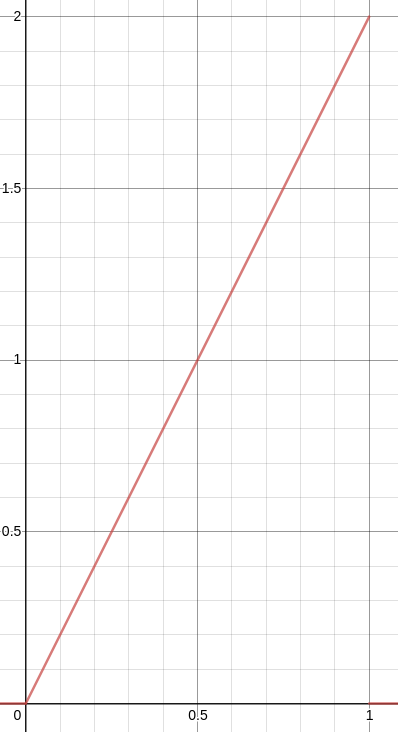
\includegraphics[width=.4\textwidth]{capture.png}}\end{center}

It looks like students tend to finish later. It is impossible to finish the exam in 0 or less minutes. It is also impossible to finish the exam in more than 1 hour.

\medskip
\noindent{\bf 3.}
\begin{align*}
    \mathbb P(X < {\frac12}) &= F_Y({\frac12}) \\
                       &= {\frac12}^2 \\
                       &= {\frac14}
\end{align*}

\newpage
\noindent{\bf 4.}
Let $A$ be the event that Clark finishes in less than half an hour. Let $B$ be the event that he is still working at the 15 minute mark.
\begin{align*}
    \mathbb P(A|B) &= \frac{\mathbb P(A \cap B)}{\mathbb P(B)} \\
                   &= \frac{F_Y({\frac12}) - F_Y({\frac14})}{1 - F({\frac14})} \\
                   &= \frac{\frac14 - \frac1{16}}{1 - \frac1{16}} \\
                   &= \frac15
\end{align*}
\end{document}
